\documentclass[10pt]{article}
\usepackage[colorlinks=true,linkcolor=black,urlcolor=black,citecolor=black]%
{hyperref}
\usepackage{cleveref}
\usepackage[natbib,citestyle=authoryear]{biblatex}
\usepackage{calc}
\usepackage{ifthen}
\usepackage{tikz}

\addbibresource{next.bib}

%adapted from http://www.texample.net/tikz/examples/pie-chart/
\newcommand{\slice}[3]{
  \draw[thick,fill=#3] (0,0) -- (#1:1) arc (#1:#2:1) -- cycle;
}

\title{The Next 700 Type Systems}
\author{Carlo Angiuli}
\date{March 31, 2017}

\begin{document}
\maketitle

Type systems classify programs in a way that enables compositional reasoning
about their behavior. As a result, type systems have found a place as one of the
major organizing principles of modern programming languages; much programming
language research focuses on new ways of classifying programs in order to
capture more sophisticated invariants, including dependent, gradual, refinement,
linear, intersection, and existential types.

However, I feel that modern type systems focus too narrowly on
\emph{classification}, which is but one of the twenty-one definitions of the
noun \emph{type} in the Oxford English Dictionary. This myopic view of types has
impeded the vast majority of the possible subdisciplines of type theory, as
depicted in \Cref{fig:pie-chart}.

\begin{figure}[hb]
\centering
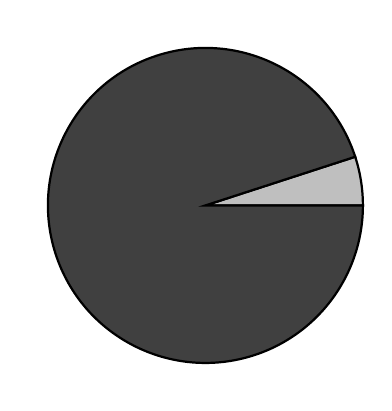
\begin{tikzpicture}[scale=2]
\slice{0}{5/100*360}{black!25}
\slice{5/100*360}{360}{black!75}
\end{tikzpicture}
\caption{95.2\% of the definitions of \emph{type, n.}, have not been explored in
the context of type systems.}
\label{fig:pie-chart}
\end{figure}

In the remainder of this paper, we describe a family of unimplemented type
systems that is intended to span differences of meaning by a group of disparate
frameworks \citep{landin66}.

\paragraph{Symbol, emblem.}

This sense of type theory is also known as \emph{symbology}, a lesser-known
field whose most famous researcher is Robert Langdon \citep{brown00}. Although
Langdon has found success focusing his efforts toward the Illuminati and
Catholic Church, it appears that other, less dangerous applications of symbology
remain underexplored.

\paragraph{A pattern stamped onto the face of a coin.}

In this sense, type systems are methods of stamping patterns on coins. The
earliest type systems required manually hammering a piece of metal between two
dies. Improvements in metalworking and industrial technologies has enabled
extensive automation in modern type systems. A recent theoretical advance in
type systems occurred during the 2013 United States debt-ceiling crisis, in
which some economists suggested that the United States Treasury could mint a \$1
trillion platinum coin in order to keep the government afloat without raising
the debt ceiling \citep{matthews13}.

\paragraph{Tip.}

The theory of tips was famously studied by medieval theologians, who sought to
compute the number of angels that could simultaneously dance on the head of a
pin. (Although this has not been experimentally validated, \citet{aquinas}
suggested that two angels cannot be in the same place.) While there are no known
applications of tip theory, advances could lead to new transistor technologies.
Unfortunately, funding sources are unlikely to surface.

\paragraph{A small block bearing a raised character, for use in printing.}

Modern type systems were invented by Johannes Gutenberg in 1440, and within
decades, made an enormous impact on European society. I suggest that programming
language researchers take credit for this early technological breakthrough in
type systems.

\paragraph{The sort of person to whom one is attracted (\emph{one's type}).}

It is well-known that types are (perhaps most) useful as tools for specifying
interfaces at abstraction boundaries. Types also, apparently, apply at
attraction boundaries; further research is warranted.

\paragraph{Printed characters (\emph{in type}).}

\TeX{} is the most popular type system among traditional type theorists. When
coupled with its large ecosystem of packages, \TeX{}'s type system is both
expressive and aesthetically-pleasing, contrary to the popular belief that it
has no types, and in fact lacks any facilities for abstraction.

\paragraph{An imperial edict released by Emperor Constans II in AD 648
prohibiting discussion of monothelitism.}

The Type of Constans was a ban on the debate between monothelitism and
dyothelitism---whether Jesus Christ, having both divine and human nature,
possessed a single will, or two wills (divine and human).

In fact, traditional type systems are already ideal for restricting inquiry into
the nature of things; recall, for instance, the fable of Professors Descartes
and Bessel in \citet{reynolds83}. To a programming language researcher, it is
clear that the Type of Constans is parametrically polymorphic in the will of
Christ, and the prohibition of discussion is simply a free theorem
\citep{wadler89}.

\paragraph{The specimen originally used to name a species (\emph{type
specimen}).}

This is clearly just a mode of use of singleton types; given a specimen $s$, its
species is the denotation of the type $S(s)$ of all specimens equal to $s$.

\paragraph{\emph{type, v.} To write with a keyboard.}

Although debate rages on over which type system is best---QWERTY, Dvorak,
Colemak, et cetera---most evidence remains anecdotal. This debate has not
impacted the success of QWERTY and its close relatives \citep{noyes83}, but the
field is nevertheless in dire need of rigorous theoretical study. Given the
relevance of keyboards to both proving and programming, I suggest submitting
research on this subject to the annual TYPES International Conference on Types
for Proofs and Programs.

\printbibliography

\end{document}
